\iffalse
\let\negmedspace\undefined
\let\negthickspace\undefined
\documentclass[journal,12pt,twocolumn]{IEEEtran}
\usepackage{cite}
\usepackage{amsmath,amssymb,amsfonts,amsthm}
\usepackage{algorithmic}
\usepackage{graphicx}
\usepackage{textcomp}
\usepackage{xcolor}
\usepackage{txfonts}
\usepackage{listings}
\usepackage{enumitem}
\usepackage{mathtools}
\usepackage{gensymb}
\usepackage{comment}
\usepackage{tikz}
\usepackage[breaklinks=true]{hyperref}
\usepackage{tkz-euclide} 
\usepackage{listings}
\usepackage{gvv}
\def\inputGnumericTable{}
\usepackage[latin1]{inputenc}                              
\usepackage{color}                                            
\usepackage{array}                                            
\usepackage{longtable}                                       
\usepackage{calc}                                             
\usepackage{multirow}   
\usetikzlibrary{circuits.ee.IEC}
\usepackage{hhline}                                           
\usepackage{ifthen} 
\usepackage{circuitikz}
\usepackage{lscape}
\newtheorem{theorem}{Theorem}[section]
\newtheorem{problem}{Problem}
\newtheorem{proposition}{Proposition}[section]
\newtheorem{lemma}{Lemma}[section]
\newtheorem{corollary}[theorem]{Corollary}
\newtheorem{example}{Example}[section]
\newtheorem{definition}[problem]{Definition}
\newcommand{\BEQA}{\begin{eqnarray}}
\newcommand{\EEQA}{\end{eqnarray}}
\newcommand{\define}{\stackrel{\triangle}{=}}
\theoremstyle{remark}
\newtheorem{rem}{Remark}
\begin{document}

\bibliographystyle{IEEEtran}
\vspace{3cm}

\title{GATE-2023 BM Q-42}
\author{EE23BTECH11207 -KAILASH.C$^{*}$% <-this % stops a space
}
\maketitle
\newpage
\bigskip

\renewcommand{\thefigure}{\theenumi}
\renewcommand{\thetable}{\theenumi}
In the circuit shown below, it is observed that the amplitude of voltage across the resistor is the same as the amplitude of the sorce voltage. What is the angular frequency $\omega_0\brak{in rad/s}$?
\begin{circuitikz}[american]
    \draw (0,0) to[R, l=$10K\Omega$] (2,0) to[L, l=$10mH$] (4,0) to[C, l=$1\mu{F}$] (6,0) -- (6,-1) 
    to[sV, l=$100\cos\brak{\omega_0 t}$] (0,-1) -- (0,0)
    (0,-1) node[circ]{} node[left]{$+$}
    (6,-1) node[circ]{} node[right]{$-$};
\end{circuitikz}

\begin{enumerate}
    \item[(A)] $10^4$\\
    \item[(B)] $10^3$\\
    \item[(C)] $10^3\pi$\\
    \item[(D)] $10^4\pi$  
\end{enumerate} \hfill(GATE 2023 BM)
\solution
\fi

\begin{table}[h]
\begin{tabular}{|l|l|l|}
\hline
\textbf{Symbols} & \textbf{Parameters} & \textbf{Value}\\ \hline
R & Resistance & $10K\Omega$ \\ \hline
L & Inductance & $10mH$ \\ \hline
C & Capacitance & $1\mu{F}$\\ \hline
$\omega_0$ & Angular Frequency & \\ \hline
$V_s$ & Source Voltage & \\ \hline
\end{tabular}
\caption{Parameter Table}
\label{tab:gate.bm.42}
\end{table}
\\
\begin{circuitikz}[american]
    \draw (0,0) to[R, l=$10K\Omega$] (2,0) to[L, l=$10^{-2}j\omega_0$] (4,0) to[C, l=$\frac{10^6}{j\omega_0}$] (6,0) -- (6,-1) 
    to[sV, l=$100\cos\brak{\omega_0 t}$] (0,-1) -- (0,0)
    (0,-1) node[circ]{} node[left]{$+$}
    (6,-1) node[circ]{} node[right]{$-$};
\end{circuitikz}

We have:
\begin{align}
    V_R&=V_s \label{eq:421}
\end{align}
Using KVL:
\begin{align}
    V_s&=V_R+V_C+V_L\label{eq:422}
\end{align}
By using \eqref{eq:421} in \eqref{eq:422}:
\begin{align}
    V_C&=-V_L\label{eq:423}\\
    X_C&=-X_L\label{eq:424}\\
    \frac{1}{j\omega_0C}&=-j\omega_0L\label{eq:425}\\
\frac{1}{LC} &= -j^2\omega_0^{2} \label{eq:426}\\ 
\omega_0^{2}&=\frac{1}{LC}\label{eq:427}\\
\omega_0&=\frac{1}{\sqrt{LC}} \label{eq:428}\\
&=\frac{1}{\sqrt{10^{-2}\times10^{-6}}}\label{eq:429}\\
&=\frac{1}{10^{-4}}\label{eq:4210}\\
&=10^4 rad/s\label{eq:4211}
\end{align}
\begin{figure}[h]
        \centering
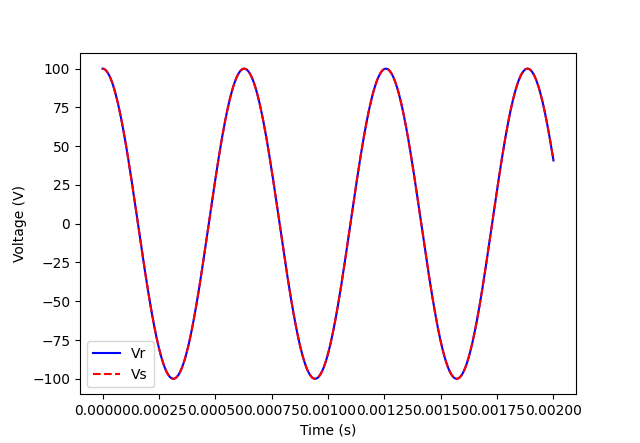
\includegraphics[width=\columnwidth]{2023/BM/42/figs/Figure42.png}
    \caption{Voltage across Resistor and Source voltage}
    \label{fig:plot42}
\end{figure}
